\section{Introduction}
\label{sec:intro}

According to the Economist, over 2.5 billion people have access to a messaging
app such as Facebook Messenger or WhatsApp. This number could reach 3.6 billion
within couple of years - half of humanity~\cite{economist}. As a result, many 
Internet firms have sought to expand their services to this canal.  In most
cases, they have done so with \emph{chatbots}, also called \emph{conversational
engines}.  Recent examples include Facebook's M and Microsoft's Tay.
Dozens of smaller businesses have also developed task-specific
alternatives, for instance to access bank services, book flights or schedule
meetings. In fact, the so-called bot economy has grown so quickly that
well-established firms such as Facebook and Russia's Telegram are now
dedicating entire marketplaces places to it. 

And indeed, chatbots have a number of advantages compared to traditional
applications. They rely on natural language, which implies a short - ideally
inexistent - learning phase.  Since they live in the user's messaging app, they
are lightweight.  They require no client installation and no maintenance.
Finally, we can easily translate their output to audio thanks with to
Text-to-Speech software, an important option for visually impaired users.

In this paper, we discuss how to engineer a chatbot to help users query large
tables.  More specifically, we focus on the interface between users and the
system. How should the users write their queries? And how should the system
answer? Our aim is to develop accessible and efficient techniques to
interrogate databases through messaging apps.  The challenges we face are
twofold. First, our medium imposes draconian restrictions on the quantity of
information that we can convey. Users expect short messages, and the support
for visuals is close to null - we can send a few pictures at most.
Furthermore, we target a casual population, that is, users with a weak
knowledge of the database and no programming skills.  Typically, we envision
distracted managers or hobbyists playing with their mobile phones.  In this
scenario, SQL is not an option.

Researchers have proposed natural language interfaces to query databases for at
least two decades~\cite{androutsopoulos1995natural, li2014constructing}. But
those solutions only solve half of the problem. They help users write queries,
but they do not help them understand their results.  They return tables of
data, as traditional database front-ends do.  But tables are neither
user-friendly nor space efficient. They can quickly saturate screens and overwhelm
users - especially on smartphones.

Another shortcoming of natural language interfaces is that they assume that
users know what they want, and they know where to find it. But in many cases,
the users' requirements are too subjective or fuzzy to be easily cast as a
query. For instance, how could we identify the ``young customers'' in a
marketing database or the ``happy countries'' is a world survey? Ideally, the
system should provide guidance. A few interfaces already offer this
feature~\cite{li2014constructing}, but they focus on the database schema (e.g.,
which columns and tables to use), not on the parameters of the query.

This paper introduces Clustine, our prototype conversational agent. Clustine
offers \emph{bi-directional} support for natural language: it collects queries,
but also summarizes their results in plain English - a research direction which
has so far received little attention in the literature. Clustine is also
\emph{proactive}.  Instead of collecting queries passively, it makes
suggestions, collects feedback and reacts accordingly.

We summarize our contributions as follows:
\begin{itemize}
    \item We introduce Clustine, a prototype chatbot based on cluster analysis
        and interactive query refinement.
    \item We present an algorithm to describe query results in a compact and
        informative fashion.
    \item We showcase Clustine with two scenarios, and validate its suggestions
        with 12 real-life datasets.
\end{itemize}
This paper is an early stage report: we present the main ideas behind Clustine
and preliminary experiments to show that they are feasible.  We will however
leave a few questions open for future research.

\begin{figure}[t]
  \centering
  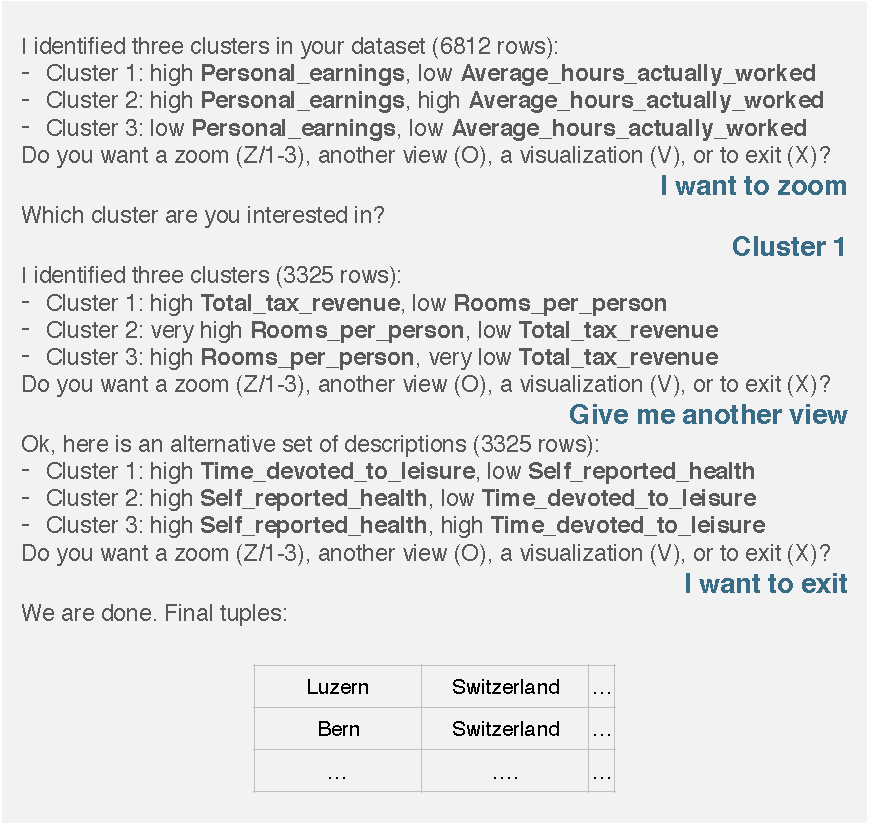
\includegraphics[width=\columnwidth]{Experiments/UseCaseIntro}
  \caption{Demonstration of Clustine.}
  \label{fig:Overview}
\end{figure}
\section{Overview}
\label{sec:overview}

Let us define our use case. Our users have access to a large table, containing
several dozen columns and 10,000s of tuples. They are interested in a small
portion of this table.  Our aim is to develop a chat-based service to help them
find and consult this interesting portion.

Our solution is based on iterative query refinement. Clustine inspects the
dataset, partitions it into a few groups, and asks the user whether they are
interested in one of the partitions. If the answer is positive, then Clustine
``drills down'' into the selection. It splits it into even smaller groups and asks for
more feedback.  If the answer is negative, then Clustine generates an
alternative set of suggestions, and it repeats the cycle.  To partition the
database, Clustine relies on \emph{cluster analysis}. It forms groups such that
similar items are gathered and different items are separated.  Thanks to this
method, it can provide coherent options: each partition effectively covers one
``family'' of tuples~\cite{sellamTKDE}.
%This method is inspired by Blaeu~\cite{sellamTKDE}, a previously
%published data analysis system based on visualizations.

Let us illustrate this process with an example. We have access to a database of
socio-economic indicators, describing a few thousand regions of the world.  Our
aim is to find the countries with the ``best conditions of life'', a purposely
ill-defined task.  Figure~\ref{fig:Overview} illustrates how to build the query
with Clustine.  It shows our system's main operations: 
\begin{itemize0}
    \item Zoom into one or several partition to refine the selection of
        tuples. 
    \item Request an alternative description of
        the partitions, to get another view of the data.
    \item Request a visualization of the partitions, to be sent as an
        image (we demonstrate this feature in
        Section~\ref{sec:demo}).
    \item Exit: Clustine closes the conversation and returns
        a sample of the selected tuples.
\end{itemize0}
Observe how our method differs from the usual query-result paradigm. Classic
database front-ends rely on open questions. The users face a ``blank page'',
and they must build their query from scratch.  With Clustine, the system
generates a sequence of closed, multiple choice questions. These
statements have two roles. First, they summarize the current selection tuples,
as they identify and describe its main components. Thus, they offer a
text-based alternative to tables and graphics. Second, they provide options for
query refinements. They let the users compose complex queries without a writing
a single line of SQL.


\section{Architecture}
\label{sec:architecture}

\begin{figure}[t!]
  \centering
  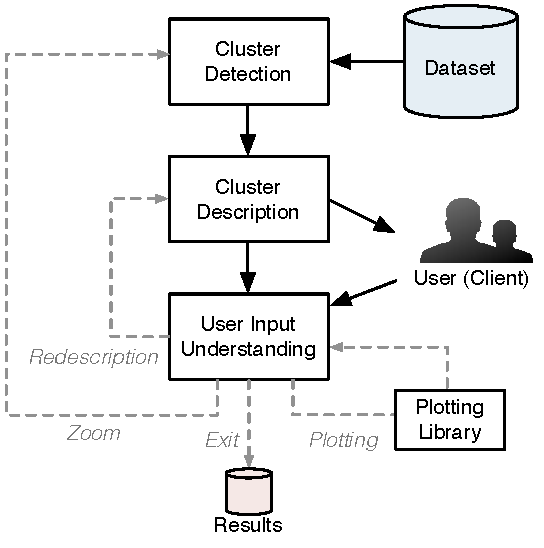
\includegraphics[width=.7\columnwidth]{Architecture}
  \caption{Overview of Clustine's Architecture.}
  \label{fig:architecture}
\end{figure}

Figure~\ref{fig:architecture} presents Clustine's architecture.  Our system
relies on three components. The first component takes a sample of tuples from
the database and detects clusters. The second one generates textual synopses of
these clusters. The last component collects the users' input and infers what
action to carry out next. We implemented the first and last stages with
well-known techniques, which we briefly discuss in this section. Designing the
second module, which generates text from clusters, was more challenging. We
tackled it with an original framework, described in Section~\ref{sec:describingClu}.

\textbf{Cluster Detection.} In principle, we could implement clustering with
any method from the literature. In practice, we opted for the EM algorithm, a
generalized variant of k-means~\cite{bishop2001bishop}. This algorithm can deal
with mixed data types and missing values. Furthermore, it returns the mean
vector and covariance matrix associated with each cluster. We will exploit this
information extensively in the description phase. To determine the number of
partitions, we use Bayesian Information Criterion~\cite{bishop2001bishop}, a
well established method from the literature. To ensure that the descriptions
are compact, we set a low cap on this value (e.g., 3 or 4). This approach
causes no loss of generality: the smaller clusters do not disappear, they
simply appear later in the exploration.

\textbf{Input Understanding.}  We implemented this module with a Naive Bayes
classifier~\cite{bishop2001bishop}, trained on a manually generated corpus to
recognize which action the user is asking for. We encode the data with bags of
words, after lower casing and stemming.  When the users request zooms, we
extract the cluster numbers with regular expressions.

\section{Describing Clusters}
\label{sec:describingClu}

\begin{figure}[t!]
  \centering
  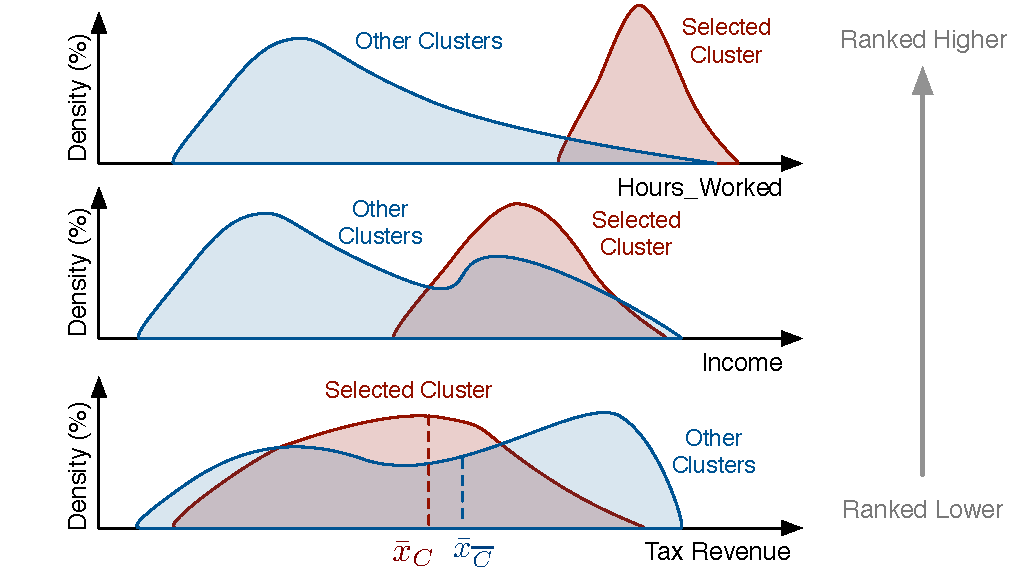
\includegraphics[width=\columnwidth]{Ranking}
  \caption{Clustine seeks variables on which the cluster are
  well separated.}
  \label{fig:Ranking}
\end{figure}

We now turn to an important challenge in our study : how to describe a set of
partitions with natural language? The EM algorithm defines each cluster by
its center (i.e., vector of means) and its covariance matrix.  But this
information is difficult to interpret. For a start, it involves all the columns
in the database. When the data contains dozens or hundreds of variables,
mentioning them all clutters the screen and overwhelms the users.
Furthermore, novice users may not be comfortable with raw data.  They may
prefer high level magnitude judgments (e.g., ``Your data has high values for
Income'') rather than literal numbers  (e.g., ``The average value for Income is
42.5 and the variance of 0.4''). This section discusses Clustine's editorial
choices, that is, which columns it uses to describe the clusters, and how it
conveys the values of the subsequent tuples.

\textbf{Ranking Variables.} To describe the clusters, Clustine uses few columns
only. More specifically, it identifies ``high contrast'' variables, that is, variables
on which the tuples in the cluster are different from those in the rest of the
data. We illustrate this idea with Figure~\ref{fig:Ranking}.  

To quantify the contrast associated with each variable, our system uses Cohen's
$d$, from the classic statistics literature~\cite{cohen1977statistical}.
Consider a cluster $C$. Let $\bar{x}_C$ (resp.  $\bar{x}_{\overline{C}}$)
describe the mean of the variable $x$ for the tuples inside (resp. outside)
the cluster.  The variable $s$ is the pooled standard deviation of the two
sets. We define Cohen's $d$ as the scaled difference between the means.
Formally:
$$
d = \frac{\bar{x}_C -\bar{x}_{\overline{C}}}{s}
$$
Admittedly, Cohen'$d$ is not the most versatile measure of statistical
dissimilarity. More sensitive alternatives exist, such as the Kullback-Leibler
divergence~\cite{bishop2001bishop}.  But this indicator is practical.
It is based on means and variances, which we obtain ``for free''
from the EM algorithm. Also, its sign and magnitude are directly interpretable. A
positive value implies that the tuples in the cluster have a higher value than
those in the rest of the database, while a negative value indicates that the
tuples have a low value on the chosen variable. A high magnitude indicates a
large deviation, while a low magnitude describes small variations. Thus,
we can exploit Cohen's $d$ directly to generate textual descriptions.

\begin{figure}[t!]
  \centering
  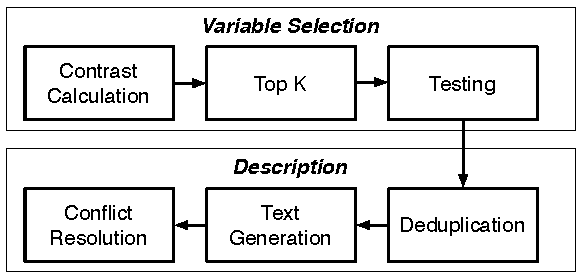
\includegraphics[width=.7\columnwidth]{Explanations}
  \caption{Workflow of Clustine's cluster description module.}
  \label{fig:descriptions}
\end{figure}

\textbf{Cluster description pipeline.} Figure~\ref{fig:descriptions} presents
Clustine's description pipeline. During the first step, our system computes the
contrast associated with each variable. It ranks them and selects the
top $K$, for some arbitrary $K$. Then it checks if the results are
statistically significant, that is, how likely it is that they were caused by
chance. By default, it uses t-tests, the counterpart of Cohen's $d$ in the
hypothesis testing literature~\cite{cohen1977statistical}. It discards the
variables associated with a low confidence. Once this process is completed,
Clustine produces the textual explanations. It first deduplicates the
variables, as explained in the following paragraph. It then generates text, using handcrafted
rules and regular expressions.  Finally, it resolves conflicts. The aim
of this phase is to detect and hierarchize the clusters that have with the
same description. For instance, if two partitions have the label ``High
income'', Clustine detects  which one covers the highest values and renames it
to ``Very high income''.

\textbf{Deduplication.} Our variable ranking scheme can lead to redundancy.
For instance, this problem can occur when several columns contain the same data
under different names or encodings (e.g., ``Income'', ``IncomeCode'' and
``IncomeCategory''). To solve it, Clustine deduplicates the columns.  It does
so in three steps. First, it obtains the correlation between every pair of
variables from the output of the EM algorithm. Second, it detects clusters of
correlated columns, using a distance-based clustering algorithm, such as
hierarchical clustering or PAM~\cite{bishop2001bishop}.  Finally, it selects
one representative column for each cluster. 

The deduplication step enforces that the results are diverse, but it can yield
losses of accuracy, described in Section~\ref{sec:eval}.  We leave it as an
option, to be chosen by the user.

\textbf{Redescription.} If the users are not satisfied with the description of
the clusters, they can request an alternative one. Then, Clustine inserts the
current selection of variables in an exclusion list and reruns the whole
pipeline described in Figure~\ref{fig:descriptions}. To save time, it reuses
intermediate results from the previous iterations, such as the contrast
scores.

\section{Use Cases}
\label{sec:demo}

\begin{figure}[t!]
  \centering
  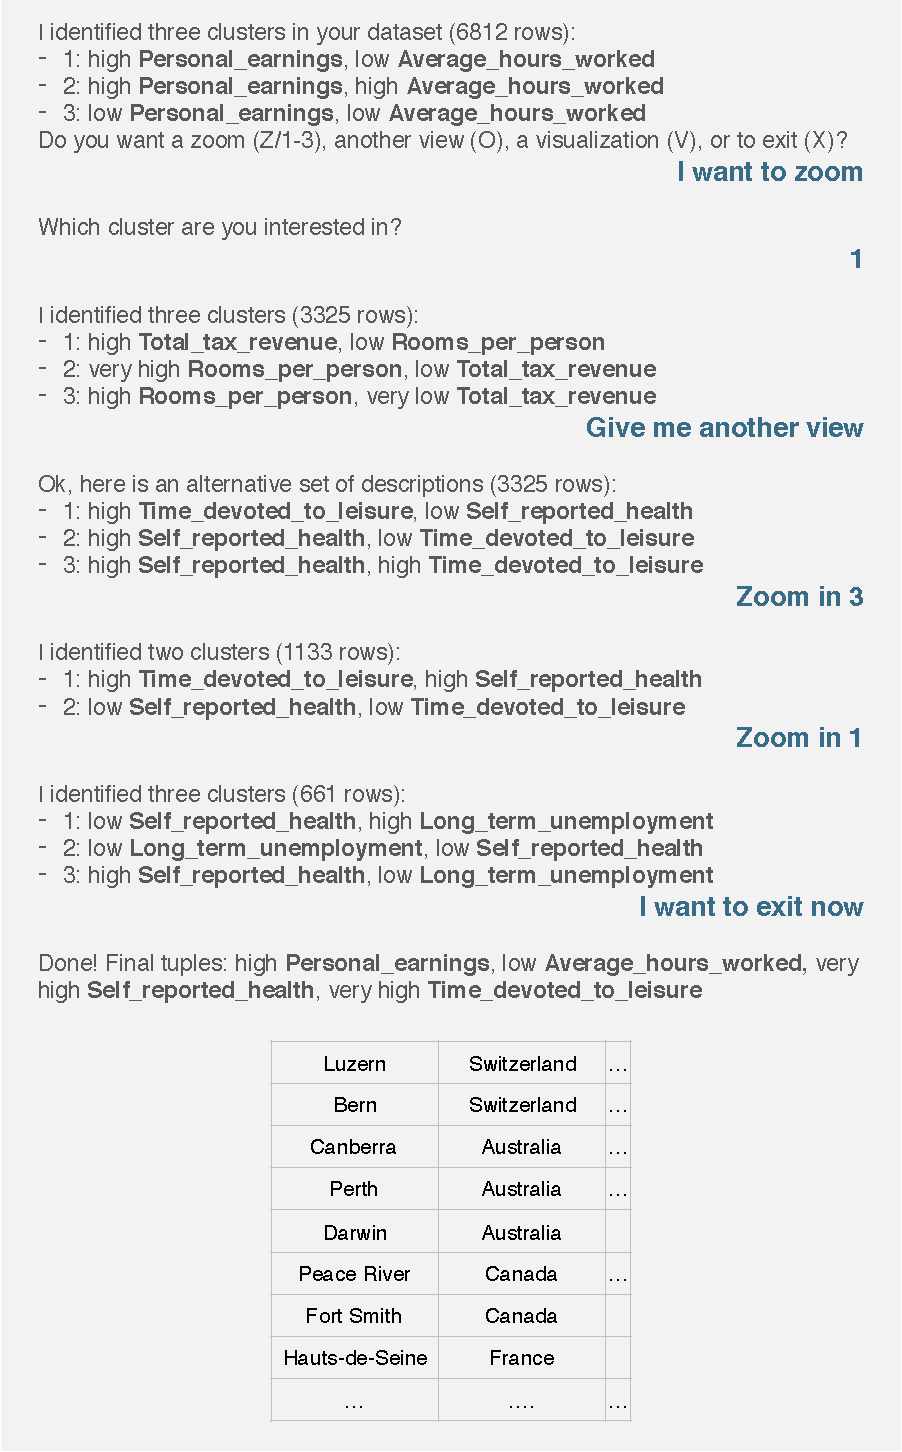
\includegraphics[width=\columnwidth]{Experiments/UseCaseFull}
  \caption{Demonstration 1: the OECD dataset.}
  \label{fig:UseCase1}
\end{figure}

\begin{figure}[t!]
  \centering
  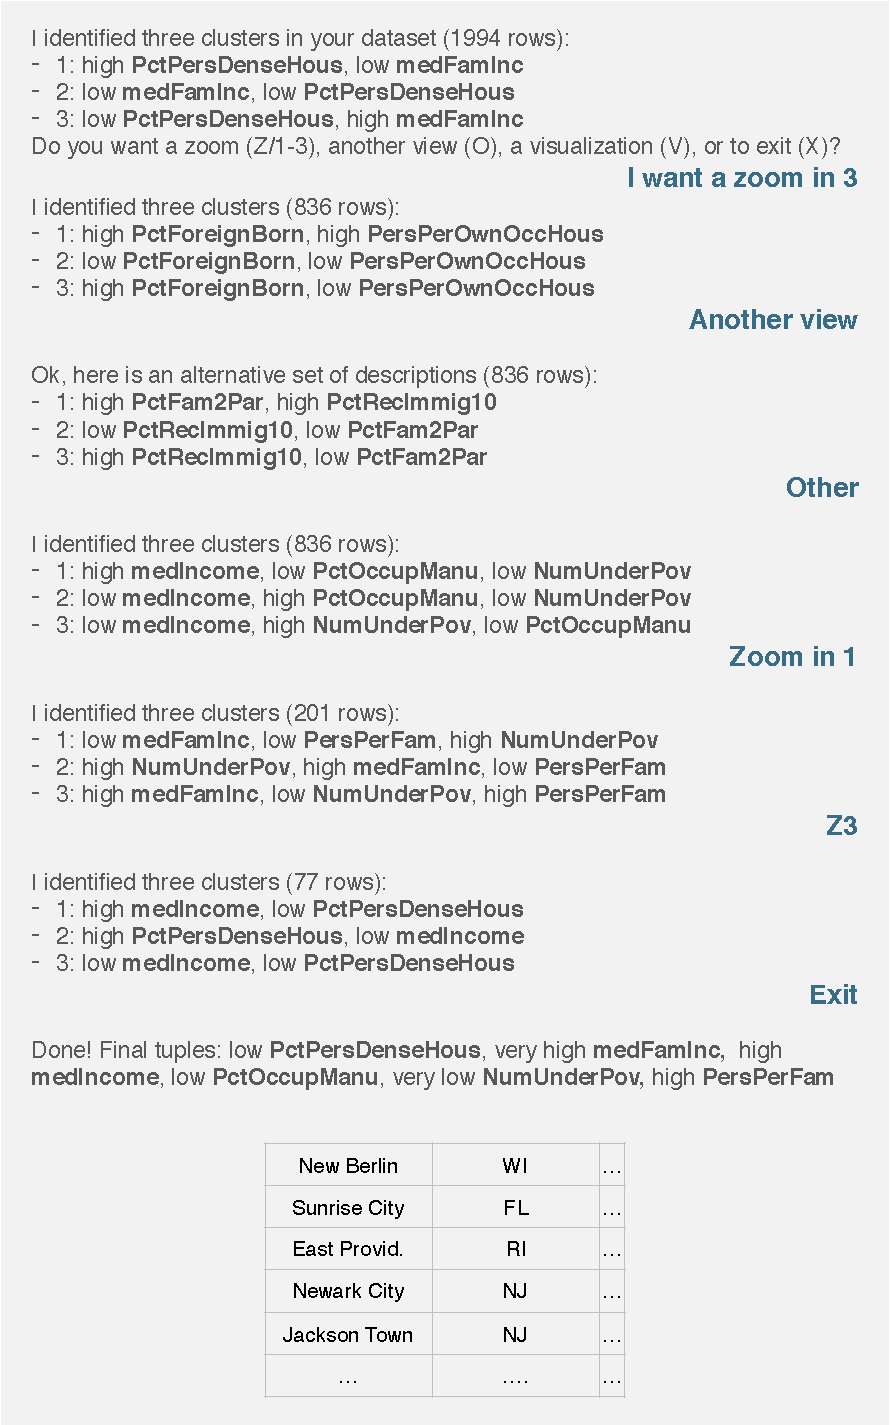
\includegraphics[width=\columnwidth]{Experiments/UseCase2}
  \caption{Demonstration 2: cities, crime and wealth in the US.}
  \label{fig:UseCase2}
\end{figure}
\begin{figure}[t!]
    \centering
    \begin{subfigure}[b]{0.48\columnwidth}
        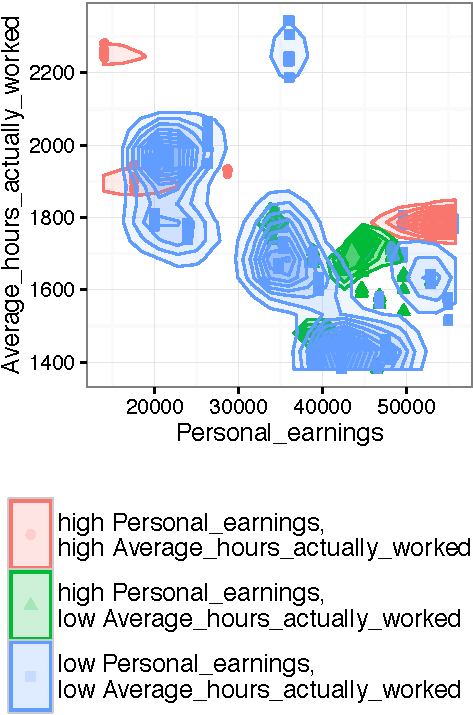
\includegraphics[width=\textwidth]{Experiments/CaseValidationResized1}
        \caption{OECD dataset, first view.}
        \label{fig:validation1}
    \end{subfigure}
    ~
    \begin{subfigure}[b]{0.48\columnwidth}
        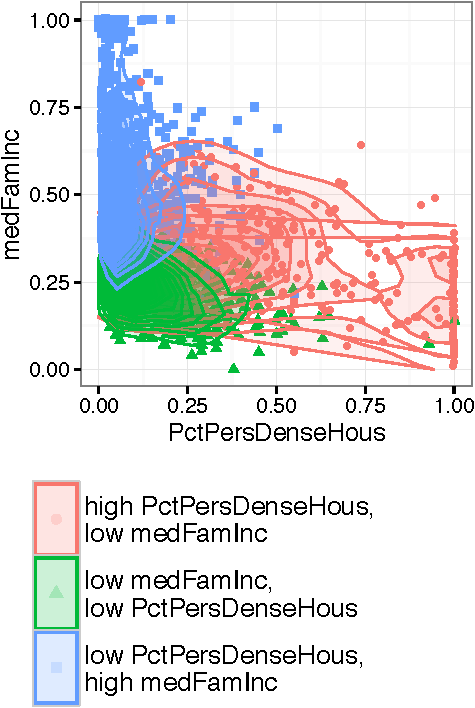
\includegraphics[width=\textwidth]{Experiments/CaseValidationResized2}
        \caption{Crime dataset, first view.}
        \label{fig:validation2}
    \end{subfigure}
%    ~
%    \begin{subfigure}[b]{0.25\textwidth}
%        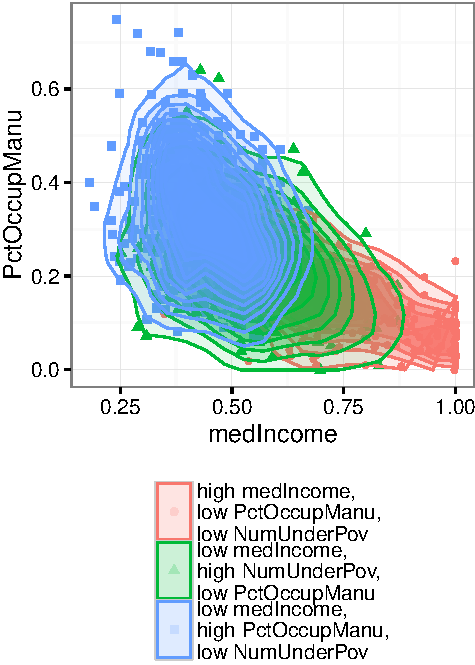
\includegraphics[width=\textwidth]{Experiments/Case2Validation8}
%        \caption{A mouse}
%        \label{fig:validation3}
%    \end{subfigure}
    \caption{Two-dimension views of Clustine's suggestions.}\label{fig:propvis}
\end{figure}

Let us demonstrate Clustine with two real-life scenarios.  We start with the
full version of our running example. The database comes
from the OECD, an international economic
organization\footnote{http://stats.oecd.org/}. It describes economic, social
and well-being indicators for 2,180 regions in 31 countries, across three
years. In total it contains 6,823 rows and 519 columns. Our aim is the find the
countries with the ``best living conditions'', a purposely vague and subjective
task.

Figure~\ref{fig:UseCase1} shows our interaction with Clustine. We exploited
three of its five suggestions. First, we selected the regions with the highest
salaries and the lowest number of hours worked.  We then refined our selection
with attributes related to leisure time, health, then unemployment. Observe
that Clustine's second suggestion was irrelevant to us. We simply discarded it by
requesting a new view.

Our second scenario is based on the Crime and Communities dataset, from the UCI
repository\footnote{http://archive.ics.uci.edu/ml/}. The data contains 128
crime and socio-economic indicators for 1,994 US cities. Our aim is to find the
richest communities. Figure~\ref{fig:UseCase2} represents the system's output
and our answers. We narrowed our selection down to 77 rows using columns
related to housing, incomes and family structure. A few of the variables were
obvious to us, such as \texttt{medIncome}. But we discovered a few others
through Clustine's suggestions. Examples of those are \texttt{PctOccupManu},
which describes the proportion of people employed in manufacturing, or
\texttt{PctPersDenseHousing}, which reports the number of houses with more than
1 person per room.

%Unfortunately, this use case also highlights a limit of Clustine: it assumes
%that the database's column names are self-explanatory. This
%assumption does not always hold, and we leave this problem open for future work.
After each suggestion, Clustine gives the option to visualize how it partitions
the data. The aim is to let users perform ``sanity checks'' and obtain more
details.  Figure~~\ref{fig:propvis} presents two of those visualization. In
both cases, we observe that the labels of the clusters match their position in
the attribute space, as expected.


\begin{figure*}[t]
  \centering
  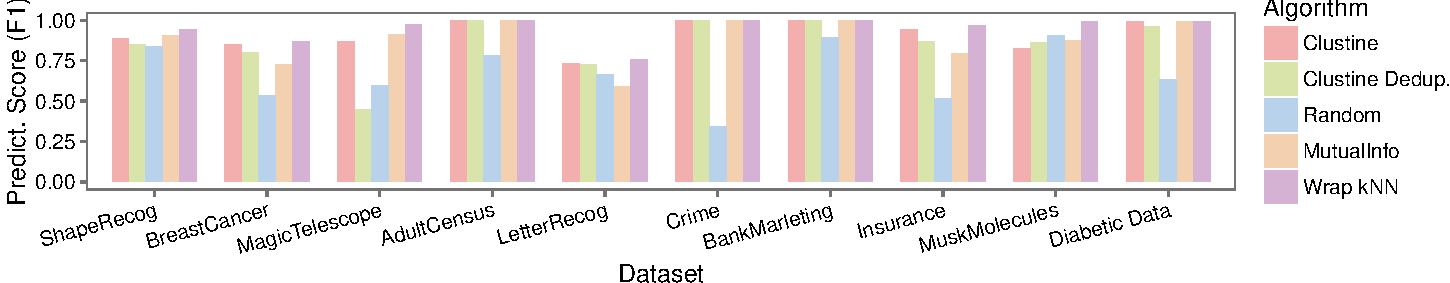
\includegraphics[width=\textwidth]{Experiments/F1_Scores}
  \caption{Accuracy of the variable selection algorithms. Higher is better.}\label{pic:accuracy}
\end{figure*}
\begin{figure*}[t]
  \centering
  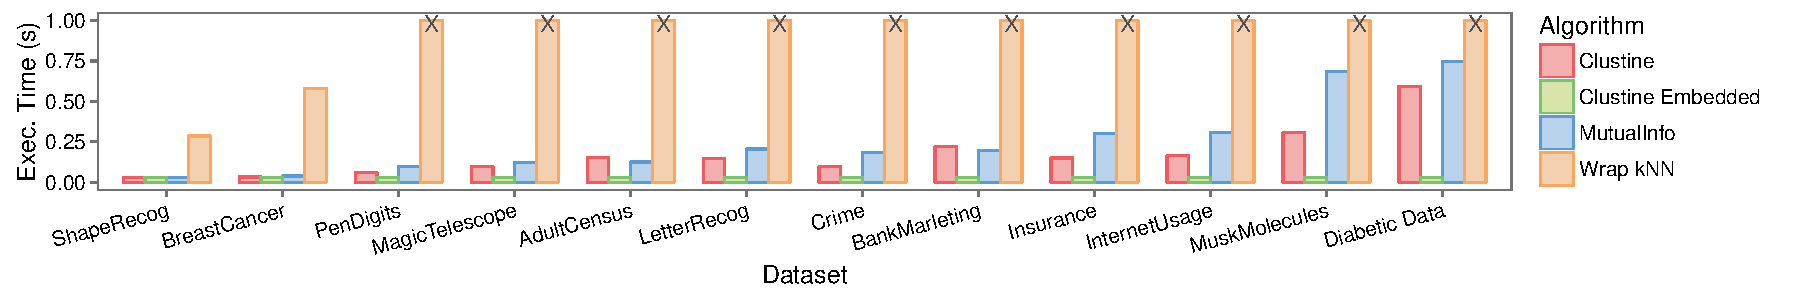
\includegraphics[width=\textwidth]{Experiments/Timings}
  \caption{Execution time of the variable selection algorithms. Lower is
  better.}
  \label{pic:runtime}
\end{figure*}

\section{Validation of the Descriptions}
\label{sec:eval}
To be efficient, Clustine must detect meaningful clusters, describe them
accurately and do so with a low latency.  Achie\-ving the first objective
depends entirely on the clustering algorithm.  Because we used EM, a well-known
method~\cite{bishop2001bishop}, we will not discuss this aspect further in this
paper. We will however evaluate how Clustine describes the clusters. More
specifically, we will focus its column selection strategy. We will check if the
columns used to describe the clusters are indeed ``informative'', and we will
measure how fast Clustine can detect them. All our  experiments are based on 12
datasets from the UCI repository, described in Table~\ref{tab:datasets}.

Our system is a MacBook Pro with an 2.6 GHz Intel Core i5 processor and 8~GB
main memory. We wrote our code in R, exploiting its native C primitives for
common operations (e.g., computing covariance matrices) and our own C library
for information theoretic operations (used in one of the baselines).

\begin{table}[!t]
    \centering
    \scriptsize
    \begin{tabular}{r c c c c} 
        \hline
        Dataset & Columns & Rows\\
        \hline
        ShapeRecog & 16 & 180\\
        %Glass & 8 & 226\\
        %Vowels &  9&1,000  \\
        BreastCancer & 34 & 234\\
        PenDigits & 17 & 7,496\\
        MAGICTelescope & 11 & 19,022\\
        AdultCensus & 14 & 32,578\\
        LetterRecog & 16 & 20,000\\
        Crime & 128 & 1,996\\
        BankMarketing & 17 & 45,213\\
        Insurance & 86 & 5,900\\
        InternetUsage & 70 & 7,463\\
        MuskMolecules & 167 & 6,600\\
        Diabetic Data & 11 & 101,818\\
        \hline
    \end{tabular}
    \caption{Characteristics of the datasets.}
    \label{tab:datasets}
\end{table}



\subsection{Accuracy of the Column Selection}
\label{sec:accuracy}
To evaluate the quality of Clustine's column selection algorithm, we exploit
statistical classifiers. We first cluster the whole database with the EM
algorithm - as our system does. We obtain one cluster label for each tuple. We
then reduce the dataset, by selecting only the columns mentioned by Clustine.
We train a classifier to infer the cluster labels from this reduced dataset.
If this operation succeeds, then we conclude that the columns are instructive:
the projection contains the information necessary to reconstitute the structure
of the whole data.  Oppositely, if the classifier fails, then the chosen
columns probably give a poor view of the data's overall distribution.
Technically, we used 5-Nearest Neighbors classifiers. We chose those for their
simplicity and efficiency.  We measure the prediction accuracy with the F1
score on 5-fold cross validation.  Higher is better.

We benchmark two variants of Clustine's column selection algorithm: with and
without deduplication, respectively denoted \texttt{Clustine} and
\texttt{Clustine Dedup}. Since we built our system for real-time interaction we
target speed. Our objective is to be as fast as possible while maintaining a
competitive accuracy.  We compare our algorithms to four baselines. The first
baseline, \texttt{Full Space}, returns all the columns in the data set. The aim
is to measure how much information Clustine loses during the column selection
process. Our hope is that this loss is as small as possible. The second and
third baselines come from the classic feature selection
literature~\cite{guyon2003introduction}.  \texttt{MutualInfo} computes the
Mutual Information (i.e., statistical dependency) between each column and the
vector of cluster labels, and it retains the top $K$ variables. We chose this
algorithm because it is fast and reasonably accurate. \texttt{Wrap kNN} choses
columns greedily, picking at each step those that yield the best classification
score with a 5-NN classifier. This method is very accurate, but also very slow.
Finally, we implemented a random baseline to ensure that the results are worth
the effort.  By default, we set $K=3$. We run each experiment five times and
average the results. 

Figure~\ref{pic:accuracy} presents the accuracy of each method. We observe that
\texttt{Full Space} dominates all the other algorithms.  Indeed, selecting
columns induces a loss of information, this is the downside of compressing the
results.  Nevertheless, the loss is neglectable on half of the datasets, and it
is less than 5\% away from the best competitor in the other cases. In our
scenario, this penalty is acceptable. The method \texttt{Wrap kNN} comes close
second, which shows that detecting small and informative sets of variables is
possible. However, this high accuracy comes with a considerable runtime
penalty, as we will show in the next section.  The methods \texttt{Clustine}
and \texttt{MutualInfo} respectively come third and fourth, with a weak
advantage for the former (\texttt{Clustine}'s score is equivalent or better in
10 cases out of 12). The algorithm \texttt{Clustine Dedup.} comes next, and
\texttt{Random} comes last. We conclude that \texttt{Clustine} is not the most
accurate framework, but it is competitive: it is at least good as
\texttt{MutualInfo}, a well established feature selection algorithm.  However,
the deduplication incurs a loss accuracy, because it drops potentially
predictive variables.
%\subsection{Diversity of the Columns}
%\label{sec:diversity}
%
%\begin{figure*}[t]
%  \centering
%  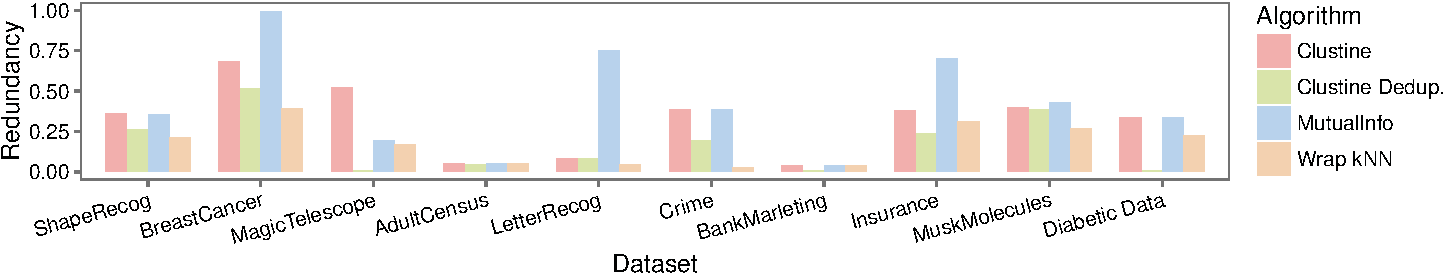
\includegraphics[width=.8\textwidth]{Experiments/Red_Scores}
%  \caption{Mean pairwise correlation between the columns of the view. Higher
%  indicates more redundancy. Lower indicates more diversity.}
%  \label{pic:dedup}
%\end{figure*}
%
%Our aim is to evaluate whether Clustine's optional deduplication step
%``works'', that is, whether it removes the redundancy in the results.
%Figure~\ref{pic:dedup} presents our results. To measure redundancy, we compute
%the pairwise correlation between the columns in the results, reverse the
%negative correlations, and computed the average. A high score indicates that
%all the columns are strongly mutually dependent, and therefore the results
%contain redundancy. A low score indicates that the columns are independent, and
%therefore the results are diverse.
%
%In all cases, our strategy works: \texttt{Clustine Dedup.} does indeed yield
%more diverse results than \texttt{Clustine}. However, there exists a few cases
%in which \texttt{Wrap-kNN} yields even more diversity. We explain this results
%with \texttt{Wrap-kNN}'s largest search space - which, we will see, also leads
%to much higher execution times.
%

\subsection{Runtime of the Column Selection}
\label{sec:speed}

We present the results of our runtime experiments in Figure~\ref{pic:runtime}.
In all cases, \texttt{Clustine} is very fast, as it is comparable to or much
faster than \texttt{MutualInfo}, an already fast algorithm. Since both
algorithms scale linearly with the number of rows and columns, the difference
comes from the constant factors. Computing and comparing means and variances
is faster than estimating mutual informations (both operations were
implemented in C).

%Figure~\ref{pic:runtime} also shows the runtime penalty incurred by the
%deduplication. If the data contains relatively few columns, then the
%performance of \texttt{Clustine Dedup.} is equivalent to that of
%\texttt{MutualInfo} - a fast algorithm. But the deduplication take more time
%with large data sets, such as \texttt{Musk Molecules}. 

To measure Clustine's runtime, we accounted for the time necessary to compute
the mean and variance of each column. But this measurement is very pessimistic.
In practice, we obtain this information directly from the EM algorithm, and
therefore we can perform the column selection without even reading the data.
The bars associated with \texttt{Clustine Embedded} in Figure~\ref{pic:runtime}
show the runtime of the computations that actually occur (that is, everything
except the calculation of the means and variances, including the
deduplication). We observe that they are almost negligible. Therefore, the cost
of describing the partitions is almost entirely shared with the clustering
step.

\section{Related Work}
\label{sec:related}

\textbf{Data exploration.} During the last decade, several papers have
described systems and interfaces to support users with no precise requirements,
or no preliminary knowledge of the data. The effort is inter-disciplinary: it
involves database researchers~\cite{idreos2015overview} as well as the
visualization community~\cite{StolteTangHanrahan2002}. Among others, existing
solutions exploit sampling~\cite{agarwal2012blink},
visualizations~\cite{StolteTangHanrahan2002}, interactive query
refinement~\cite{dimitriadou2014explore}, relevance
feedback~\cite{akbarnejad2010sql} or modern interface devices such as touch
screens~\cite{jiang2015snaptoquery}. But to the best of our knowledge, no one
has ever attempted to develop a chatbot to support exploration. Our work was
inspired by Blaeu~\cite{sellamTKDE}, which also uses cluster analysis to help
users build queries. But Blaeu relies on visualizations, and it provides no
mechanism to summarize its findings. Clustine is also close to
SeeDB~\cite{vartak2015see}, which recommends database views. But SeeDB helps
users visualize the result of their queries, it does not help writing them.
Furthermore, it relies almost exclusively on visuals.

\textbf{Natural language datbase interfaces.} Authors have introduced database
interface based on natural language for at least two
decades~\cite{androutsopoulos1995natural}. Li and Jagadish's system is
probably one of the most successful example of this
effort~\cite{li2014constructing}. But these interfaces rely on the classic
query-result paradigm.  Typically, those system helps users compose SQL
statements, using schema information. In contrast, we help them understand
their results, using machine learning. Those two approaches are orthogonal. Our
work also resembles ABCD~\cite{Lloyd2014ABCD}, a natural language-based
machine learning engine. But this system focuses exclusively on regression
models, while target database queries and cluster analysis.


\section{Conclusion}
\label{sec:conclusion} 
In this paper, we presented Clustine, our prototype chatbot to help users
interrogate large tables.  Compared to existing natural language interfaces,
our system is based on inverted querying: instead of aksing the users to write
queries from scratch, the software comes up with its own suggestions. Thanks to
this paradigm, our users can compose complex queries with only a shallow
knowledge of the data, a minimal amount of characters and an end-to-end support
for natural language.

Our main priority for the future is to run extensive
user studies, in order to further evaluate and improve our system. More
generally, little to no work has addressed the problem of describing data with
natural language. We are convinced that this research direction has a bright
future ahead.

%\section{Acknowledgments}
%\label{sec:ack} 
%This work was supported by the Dutch national program COMMIT
